\chapter{Proposed Technologies}
\label{ch:design}

The problem set asks for two technologies that share a speed limit. This chapter defines them so that each can be implemented and so that each can be evaluated from the same equations the estimator in Chapter~\ref{ch:estimate} will call. Section~\ref{sec:tech1} is compliance-aware vision metering. It takes images, force and inertial measurements and returns a plate-speed command, a depth command and a set of speeds on which those commands are claimed to meet the index bounds. Section~\ref{sec:tech2} is singulation-constrained terrain model-predictive coverage. It takes the field, the elevation model and that speed set, and returns a heading and a speed profile. Neither section assumes the other has already been tuned on a prototype. Where a coefficient is numerical, it is one of the specification values in Table~\ref{tab:spec} or it is introduced here and carried unchanged into the estimation.

\section{Compliance-aware vision metering}
\label{sec:tech1}

\subsection{Role of the loop and the signals it may use}

Compliance-aware vision metering is a per-row controller. It does not steer the vehicle and it does not choose the heading. Its outputs are the plate angular speed \(\omega\), the depth-actuator set-point \(z_{\mathrm{cmd}}\), and a Boolean feasibility flag that is false when the current speed has left \(\mathcal{V}_{\mathrm{meter}}\). Its inputs are a camera frame of the plate and the upper tube, the boot force \(F_b\), the ultrasonic range \(r_u\) from a sensor on the boot to the soil, the arm pitch rate and vertical acceleration from an inertial sensor, and the ground speed \(v\) supplied by the vehicle. Ground speed is an input, not a result. That is the interface Requirement~R10 demanded.

The loop is organised in four blocks that run at different rates, because a detector and a depth servo do not want the same clock. The detector runs at the camera rate, taken as \SI{30}{Hz}, which at the design spacing and at \SI{1.5}{m/s} gives several frames per hole. A tracking filter over hole events runs at \SI{100}{Hz} so that it can timestamp a release more finely than the frame period. The depth servo runs at \SI{50}{Hz}. The feasibility flag is recomputed whenever \(v\) or the estimated vibration changes, and is sent to the coverage controller at \SI{10}{Hz}. Figure~\ref{fig:cavm} shows the blocks and the only path by which this technology is allowed to influence the vehicle: the feasible-speed message.

\begin{figure}[ht]
\centering
\begin{tikzpicture}[font=\small, node distance=0.45cm and 0.6cm, >=Stealth, box/.style={draw, rounded corners, align=center, minimum height=0.9cm, fill=blue!6}]
  \node[box] (cam) {camera\\plate and tube};
  \node[box, right=of cam] (det) {detector\\empty / single / double};
  \node[box, right=of det] (ukf) {flexure and\\release filter};
  \node[box, below=of det] (depth) {depth servo\\ \(z_{\mathrm{cmd}}\)};
  \node[box, below=of ukf] (plate) {plate law\\ \(\omega\)};
  \node[box, fill=orange!12, below=of cam] (flag) {feasible set\\ \(\mathcal{V}_{\mathrm{meter}}\)};
  \node[draw, dashed, rounded corners, align=center, right=1.1cm of plate, minimum height=1.5cm] (mpc) {SCT-MPC\\uses \(v\) only};
  \draw[->] (cam) -- (det);
  \draw[->] (det) -- (ukf);
  \draw[->] (ukf) -- (plate);
  \draw[->] (ukf) -- (depth);
  \draw[->] (ukf) -- (flag);
  \draw[->] (flag) -- (mpc);
  \draw[->] (mpc.north) |- node[pos=0.25, above] {\(v\)} (ukf.north);
\end{tikzpicture}
\caption{Compliance-aware vision metering. The vehicle is influenced only through the feasible-speed set. Plate speed and boot depth stay on the row unit.}
\label{fig:cavm}
\end{figure}

\subsection{Timber flexure as a process model}

The arm is reduced to a single degree of freedom, the vertical displacement \(\delta\) of the boot relative to the chassis reference, positive downward. With the equivalent stiffness and damping of the problem set,
\begin{equation}
\label{eq:sddot}
m_{\mathrm{eq}}\ddot{\delta} + c_d \dot{\delta} + k\delta = F_{\mathrm{soil}}(t) + F_{\mathrm{act}}(t),
\end{equation}
where \(c_d = 2\zeta\sqrt{k m_{\mathrm{eq}}}\) and \(F_{\mathrm{act}}\) is the force of the depth actuator. The actuator is modelled as a first-order lag on the command, with time constant \(\tau_z=\SI{80}{ms}\), which is deliberately slower than the resonant period. A depth loop that tries to be faster than \(f_n\) on a lightly damped flexure will need a lead term and a measurement of \(\dot{\delta}\); the inertial sensor provides that measurement, and the lag model keeps the design from claiming a bandwidth the wood cannot be asked for. Substituting the specification values gives \(c_d = 2\cdot 0.08\cdot\sqrt{8200\cdot 6.8}\approx \SI{37.8}{N\,s/m}\).

Soil force is split into a slow part and a roughness part,
\begin{equation}
\label{eq:fsoil}
F_{\mathrm{soil}} = F_0(z) + F_r \sin\bigl(2\pi s/\lambda + \phi\bigr),
\end{equation}
where \(s\) is the distance travelled and \(F_0\) depends on the nominal penetration. Godwin and O'Dogherty's family of models justifies a monotone increase of vertical force with depth \cite{godwin2007}. For the controller a local linearisation is enough,
\begin{equation}
\label{eq:flinear}
F_0(z) \approx F_0(z^{\star}) + k_{\mathrm{soil}}\bigl(z-z^{\star}\bigr),
\end{equation}
with \(k_{\mathrm{soil}}\) identified from a short calibration pass, not assumed from a national soil map. The ultrasonic range measures the distance from the boot datum to the surface. If the boot has sunk a depth \(z_{\mathrm{sink}}\) below the surface, the range and the flexure coordinate are related by a constant offset \(c_r\) that is calibrated when the machine is lowered onto a hard reference,
\begin{equation}
\label{eq:range}
r_u = c_r - \delta + n_r,
\end{equation}
where \(n_r\) is measurement noise. Equation~\eqref{eq:range} is what allows the filter to see \(\delta\) even when the inertial sensor has been integrated long enough to drift.

The transfer from a harmonic force of amplitude \(F_r\) to a displacement amplitude is \(F_r M(r)/k\), with \(M\) from Equation~\eqref{eq:mag}. This is the calculation that places the forbidden steady speed near \SI{2.4}{m/s} for \(\lambda=\SI{0.45}{m}\). It is also the calculation the filter uses as its process-noise schedule: when the estimated frequency ratio approaches one, the process noise on \(\delta\) is inflated, the filter trusts the ultrasonic range more than the open prediction, and the feasibility flag is cleared if the predicted depth variance exceeds \(\sigma_{z,\max}^2\).

\subsection{Seed state and the observation the camera actually makes}

A cell is a discrete object. The filter does not pretend otherwise by burying the cell index inside a purely continuous state. The continuous state at row \(i\), suppressing the row index until the multi-row note below, is
\begin{equation}
\label{eq:state}
\mathbf{x} =
\begin{bmatrix}
\delta & \dot{\delta} & z_{\mathrm{bias}} & t_{\mathrm{rel}} & v_{\mathrm{ex}}
\end{bmatrix}^{\mathsf{T}}.
\end{equation}
Here \(z_{\mathrm{bias}}\) is a slowly varying offset between the actuator command and the true depth, accounting for wear of the wooden pivot and for a change in surface residue. \(t_{\mathrm{rel}}\) is the predicted time of the next release relative to the current sample. \(v_{\mathrm{ex}}\) is the horizontal velocity of the seed at release in the soil frame, which Equation~\eqref{eq:carry} turns into a spacing error. The cell label \(\ell\in\{\mathrm{empty},\mathrm{single},\mathrm{double}\}\) is carried beside \(\mathbf{x}\) as a discrete mode, updated by the detector, not as a fifth continuous coordinate.

Between camera frames the continuous state is predicted by Equation~\eqref{eq:sddot} for the flexure coordinates, by \(\dot{z}_{\mathrm{bias}}=0\) plus a small process noise, and by
\begin{equation}
\label{eq:trel}
\dot{t}_{\mathrm{rel}} = -1,\qquad
\dot{v}_{\mathrm{ex}} = 0,
\end{equation}
with \(t_{\mathrm{rel}}\) reset to the predicted time of the next cell whenever a release is declared. The predicted release time of cell \(n\) under the feedforward plate speed is
\begin{equation}
\label{eq:tn}
\hat{t}_n = t_{n-1} + \frac{2\pi}{N\omega}.
\end{equation}
A nonzero \(\dot{\delta}\) at the gate changes the actual release. The correction used here is geometric. The gate is a lip of angle \(\gamma\) relative to the arm. A vertical arm velocity \(\dot{\delta}\) moves the lip across the seed and shifts the release time by
\begin{equation}
\label{eq:tshift}
\Delta t_{\mathrm{rel}} = \frac{\dot{\delta}\,\sin\gamma}{r_p\,\omega},
\end{equation}
where \(r_p\) is the radius of the cell circle. Equation~\eqref{eq:tshift} is the compliance-aware part of the vision loop. A detector that sees a seed still in the cell at a time when a rigid-body schedule expected it to have left will, without Equation~\eqref{eq:tshift}, declare a miss. With the equation, the filter first asks whether the arm velocity explains the delay. Only the residual delay is offered to the miss logic.

The detector returns a class and a confidence \(p_{\ell}\) for each visible cell. Following the published operating points, the estimation will credit the detector with a recall of \num{0.99} and a precision of \num{0.985} on the empty-versus-occupied decision when the window is clean \cite{blaser2024,zhao2025yolo}. The filter does not use those two numbers as if they were probabilities of the current frame. It uses the frame confidence, and it uses the published numbers only when Chapter~\ref{ch:estimate} averages over many seeds. A double is declared when two connected components, or two detector boxes, occupy one cell above a confidence threshold. The action is not symmetric with the empty-cell action. An empty cell can be repaired by advancing the next filled cell if Equation~\eqref{eq:latency} holds. A double already in the gate cannot be unreleased. The plate law below therefore slows the plate and raises a singulator duty, if a mechanical singulator is fitted, but it does not pretend to retrieve the extra seed.

\begin{figure}[ht]
\centering
\begin{tikzpicture}[font=\small, >=Stealth, scale=1.0]
  \draw[thick] (0,0) circle (1.7);
  \foreach \a in {0,15,...,345} {
    \fill[blue!30] (\a:1.35) circle (1.5pt);
  }
  \fill[red!70] (20:1.35) circle (2.4pt);
  \node[red!70!black] at (20:1.9) {empty};
  \draw[thick] (1.55,-0.35) -- (2.6,-1.3);
  \draw[thick] (1.85,-0.15) -- (2.9,-1.1);
  \node[align=left] at (4.0,-0.7) {wooden tube};
  \fill (2.75,-1.2) circle (1.5pt) node[right] {\ seed};
  \draw[->] (0,0) -- (0.9,0.5) node[midway, above left] {\(\omega\)};
  \draw[dashed] (0,0) -- (20:1.7);
  \node at (-2.3,1.3) {camera};
  \draw[->] (-1.7,1.15) -- (-0.4,0.55);
\end{tikzpicture}
\caption{Plate observation. The detector labels cells before they reach the gate. One empty cell is still repairable. A seed already in the wooden tube is only a measurement of release time, not a seed that can be called back.}
\label{fig:plate}
\end{figure}

\subsection{Unscented filter for a mixed observation}

The process model is nonlinear because of Equation~\eqref{eq:tshift} and because the ultrasonic geometry saturates when the boot leaves the soil. An extended Kalman filter would linearise both. An unscented filter propagates a small set of sigma points through the nonlinear map and matches the mean and covariance up to second order, which is the property Julier and Uhlmann designed it for \cite{julier1997}. Welch and Bishop's notes and S{\"a}rkk{\"a}'s text are the implementation references for the weights and the Joseph-stabilised covariance update \cite{welch2006,sarkka2013}. Thrun, Burgard and Fox discuss the same update in the setting of a robot that must stamp sensor events onto a moving base \cite{thrun2005}. The pattern here is closer to their event filter than to a simultaneous-localisation map: the ``landmark'' is the next cell, and it is consumed when the seed passes the gate.

Let \(n_x=5\) and let \(\lambda_{\mathrm{ukf}}=\alpha_{\mathrm{ukf}}^2(n_x+\kappa_{\mathrm{ukf}})-n_x\) with the usual \(\alpha_{\mathrm{ukf}}=10^{-2}\), \(\kappa_{\mathrm{ukf}}=0\). Given mean \(\hat{\mathbf{x}}\) and covariance \(P\), the sigma points are the mean and the symmetric columns of the matrix square root of \((n_x+\lambda_{\mathrm{ukf}})P\). Each point is pushed through Equations~\eqref{eq:sddot}--\eqref{eq:tshift} over one filter step \(h_f=\SI{10}{ms}\). The predicted mean and covariance are the weighted sums given by Julier and Uhlmann, with process noise \(Q\) diagonal. The diagonal entries are not constant. The entry on \(\delta\) is scaled by \(1+4\max(0, M(r)-1)^2\), so that a resonant arm is not assigned a calm process. The entry on \(t_{\mathrm{rel}}\) is scaled by the detector's reported confidence: a low-confidence frame is not allowed to pull the release time hard.

The observation vector stacks the quantities a sample actually contains,
\begin{equation}
\label{eq:obs}
\mathbf{y} =
\begin{bmatrix}
r_u & F_b & a_{\mathrm{imu}} & \mathbf{1}_{\mathrm{cross}}
\end{bmatrix}^{\mathsf{T}}.
\end{equation}
The indicator \(\mathbf{1}_{\mathrm{cross}}\) is one when the tube window sees a seed cross a fixed image row. Its predicted value is a smooth step of \(t_{\mathrm{rel}}\), \(\psi(t_{\mathrm{rel}})=(1+\exp(t_{\mathrm{rel}}/\tau_{\psi}))^{-1}\) with \(\tau_{\psi}=\SI{8}{ms}\), which restores differentiability for diagnostics even though the unscented filter does not need the Jacobian. The force observation is \(F_b = k\delta + c_d\dot{\delta} + n_F\), the inertial observation is the second derivative from Equation~\eqref{eq:sddot} divided by \(m_{\mathrm{eq}}\), and the range observation is Equation~\eqref{eq:range}. Standard unscented update equations apply. A cell label is applied after the continuous update, as a mode switch: if the label is empty and the residual of Equation~\eqref{eq:tshift} does not explain the absence, the discrete miss hypothesis is raised.

The initial covariance is set from the calibration pass: \(\delta\) within \(\SI{5}{mm}\), \(\dot{\delta}\) within \(\SI{0.05}{m/s}\), bias within \(\SI{3}{mm}\), release-time uncertainty equal to a quarter of the hole period, and exit-velocity uncertainty \(\SI{0.05}{m/s}\). Those values are priors for the filter, not results.

\subsection{Plate law and the condition for attempting a repair}

The plate command is the feedforward of Equation~\eqref{eq:rate} plus a correction that exists only when a repair is both necessary and timely,
\begin{equation}
\label{eq:plate}
\omega = \omega^{\star}(v) + \Delta\omega_{\mathrm{repair}} + \Delta\omega_{\mathrm{double}} + K_{\omega}\bigl(\hat{t}_{\mathrm{rel}} - t_{\mathrm{sched}}\bigr).
\end{equation}
The last term is a small proportional trim, with gain \(K_{\omega}\), that advances or retards the plate when the predicted release drifts from the schedule but the cell is occupied. It is saturated at \(\pm\num{8}\%\) of \(\omega^{\star}\) so that a noisy filter cannot double the seed rate. The double term \(\Delta\omega_{\mathrm{double}}\) is non-positive. It reduces plate speed for one hole period after a double is seen, on the reasoning that a double often comes from overspeed or from too much vacuum, and that the next hole should not be asked to repeat the condition. The vacuum itself, if the plate is pneumatic rather than a mechanical cell, is not placed under high-rate feedback in this design. Equation~\eqref{eq:vacuum} is used to set the nominal \(\Delta p\), including a margin for \(a_{\mathrm{vib}}\) evaluated at the largest \(M(r)\) allowed inside \(\mathcal{V}_{\mathrm{meter}}\). A slow outer trim, once per ten metres, may lower \(\Delta p\) if doubles dominate misses. Fast vacuum modulation is left out because a wooden hopper does not contain a pressure plenum that settles in one hole period.

The repair term is the one that can cause harm if it is late. Let \(\tau=\tau_v+\tau_a\) and let \(\Delta t=x_{\mathrm{ref}}/v\). Define the repair fraction
\begin{equation}
\label{eq:cfrac}
c(v,a) =
\begin{cases}
1 & \text{if }\Delta t \ge 1.35\,\tau + 0.012\,|a| + 0.030,\\
0.15 & \text{if }\Delta t \le 1.35\,\tau + 0.012\,|a|,\\
\text{linear in between.}
\end{cases}
\end{equation}
Equation~\eqref{eq:cfrac} is a design function, not a fit to a new experiment. The coefficient \(0.012\) seconds per metre-per-second-squared charges the extra time the stepper needs when the vehicle is accelerating and the scheduled \(\omega^{\star}\) is itself a moving target. The floor of \(0.15\) expresses Borja's observation that a late loop does not become a zero loop; it becomes a harmful one, so the controller should mostly stop repairing rather than repair at random \cite{borja2021}. The command is then
\begin{equation}
\label{eq:repair}
\Delta\omega_{\mathrm{repair}} =
\begin{cases}
\dfrac{2\pi}{N}\, c(v,a)\, \mathbf{1}_{\mathrm{empty}} & \text{over the next hole period,}\\
0 & \text{otherwise.}
\end{cases}
\end{equation}
When \(c=1\), an empty cell is replaced by bringing the following cell forward one pitch. When \(c\) is near the floor, the indicator is ignored and the plate stays on the feedforward. The feasibility set reported to the coverage controller is
\begin{equation}
\label{eq:vset}
\mathcal{V}_{\mathrm{meter}} = \bigl\{ v : c(v,0) \ge 0.85 \bigr\}
\setminus \bigl\{ v : M\bigl(v/(\lambda f_n)\bigr) > 3 \bigr\}.
\end{equation}
With the specification numbers, \(1.35\tau+0.030=\SI{0.107}{s}\) and \(x_{\mathrm{ref}}/v \ge 0.107\) gives \(v\le \SI{1.87}{m/s}\) for full repair authority with a margin. The magnification bound removes a neighbourhood of \SI{2.4}{m/s} even if some other spacing were to make the latency look acceptable. Both cuts are reported upward. The coverage controller does not re-derive them.

\begin{algorithm}[ht]
\caption{Plate and feasibility update on one row}
\label{alg:plate}
\begin{algorithmic}[1]
\Require speed \(v\), acceleration \(a\), filter state, detector label \(\ell\), confidences
\State \(\omega^{\star} \gets 2\pi v / (N x_{\mathrm{ref}})\)
\State predict \(\mathbf{x}\) through the flexure and Equation~\eqref{eq:tshift}
\State update \(\mathbf{x}\) with \(\mathbf{y}\) by the unscented step
\State \(c \gets c(v,a)\) from Equation~\eqref{eq:cfrac}
\If{\(\ell=\mathrm{empty}\) and residual delay is unexplained and \(c\ge 0.85\)}
  \State apply one-pitch advance over the next hole period
\ElsIf{\(\ell=\mathrm{double}\)}
  \State \(\omega \gets \omega^{\star} - \Delta\omega_{\mathrm{double}}\) for one hole period
\Else
  \State \(\omega \gets \omega^{\star} + K_{\omega}(\hat{t}_{\mathrm{rel}}-t_{\mathrm{sched}})\), then saturate
\EndIf
\State publish \(\omega\), and publish whether \(v\in\mathcal{V}_{\mathrm{meter}}\)
\end{algorithmic}
\end{algorithm}

\subsection{Depth servo}

The depth loop is a proportional-integral law on the filtered boot displacement, with a damping term on \(\dot{\delta}\),
\begin{equation}
\label{eq:depth}
\begin{aligned}
e_z &= z^{\star} - \bigl(z_{\mathrm{ref,arm}} + \hat{\delta} + \hat{z}_{\mathrm{bias}}\bigr),\\
F_{\mathrm{act}} &= K_p e_z + K_i \int e_z\,dt - K_d \hat{\dot{\delta}}.
\end{aligned}
\end{equation}
The integral state is clamped so that a long lift of the machine, when the boot is in the air and the ultrasonic return is invalid, does not wind up a force that slams the boot into the soil on the next entry. The integral is also frozen whenever the ultrasonic innovation exceeds a gate, which is the filter's way of saying that residue or a stone has produced a false range. Gains are chosen by loop shaping on Equation~\eqref{eq:sddot}. The target closed-loop bandwidth is \SI{3}{Hz}, below \(f_n=\SI{5.53}{Hz}\), so the servo removes the \SI{9.8}{mm} static deflection and the slow part of the roughness, and it does not attempt to cancel the resonant peak. Cancelling that peak with actuator force would require a bandwidth beyond the wood and would pump energy into \(f_n\). The resonant peak is rejected by the speed constraint instead. This division of labour is the central design choice of the first technology.

A short Lyapunov argument records why the constrained servo does not fight the flexure. Take the flexure energy
\begin{equation}
\label{eq:energy}
V(\delta,\dot{\delta}) = \tfrac12 m_{\mathrm{eq}}\dot{\delta}^2 + \tfrac12 k\delta^2
\end{equation}
and the actuator policy of Equation~\eqref{eq:depth} with the integral held constant. Differentiating along Equation~\eqref{eq:sddot} yields
\begin{equation}
\label{eq:vdot}
\dot{V} = -c_d\dot{\delta}^2 + \dot{\delta}\, F_{\mathrm{soil}} + \dot{\delta}\, F_{\mathrm{act}}.
\end{equation}
The damping term is negative semidefinite. \(F_{\mathrm{act}}\) contributes \(\dot{\delta}(K_p e_z - K_d\dot{\delta})\) plus the integral contribution. The \(-K_d\dot{\delta}^2\) term augments wood damping, which is the reason for the rate feedback. The proportional term exchanges energy with the depth error and is bounded because \(F_{\mathrm{act}}\) is saturated at the force of a small linear actuator, taken as \SI{120}{N} in the build. Saturation prevents a noisy \(\hat{\delta}\) from commanding more force than the timber pivot is designed to carry. Asymptotic convergence to a point is not claimed, because \(F_{\mathrm{soil}}\) is persistently exciting. What is claimed, and what the estimation checks, is that the steady component of \(\delta\) is driven inside the band and that the resonant component is left to the speed constraint.

\begin{proposition}
\label{prop:split}
Under Assumption~\ref{as:flex}, a depth loop of bandwidth below \(f_n\) together with the exclusion of \(\{v:M(r)>3\}\) from \(\mathcal{V}_{\mathrm{meter}}\) keeps the resonant mode from being both strongly excited and strongly actuated. The loop is responsible for the mean depth. The vehicle speed is responsible for the dynamic magnification.
\end{proposition}

Proposition~\ref{prop:split} is a design proposition. Its content is the separation, not a new stability theorem. Khalil's treatment of singular perturbation is the justification for controlling the slow depth error while treating the fast resonant response as a disturbance to be avoided rather than inverted \cite{khalil2002}.

\subsection{Predicted indices at a constant speed}

The coverage layer needs a miss probability it can evaluate without running the filter. The map used for that purpose is an explicit function, constructed so that its shape agrees with the qualitative findings of Section~\ref{sec:prev-meter}: misses rise with speed, rise again with acceleration, and rise when the arm magnification grows. For the open-loop plate, which is the baseline,
\begin{equation}
\label{eq:openmiss}
\begin{aligned}
\mis_{\mathrm{ol}}(v,a) &= \mathrm{clip}_{[0,0.55]}\Bigl(
0.055 + 0.085\max(0,v-0.7) + 0.040|a| \\
&\qquad + 0.0045\max\bigl(0,\, d_{\mathrm{mm}}(v)-3\bigr)\Bigr),\\
\mul_{\mathrm{ol}}(v,a) &= \mathrm{clip}_{[0,0.30]}\Bigl(
0.028 + 0.022\max(0,v-0.8) + 0.015|a|\Bigr),
\end{aligned}
\end{equation}
where \(d_{\mathrm{mm}}(v) = 10^3 F_r M(r)/k\) is the dynamic displacement amplitude in millimetres and \(\mathrm{clip}\) denotes saturation to the interval. Equation~\eqref{eq:openmiss} is not identified from a woody-seed trial. The intercept and the slopes are chosen so that, at ordinary planting speeds, the open-loop quality-of-feed index sits in the \numrange{0.75}{0.90} range that irregular seed produces on a plate that was not tuned for it, and so that the acceleration term is visible, as Mangus et al.\ found it to be \cite{mangus2017}. Chapter~\ref{ch:estimate} states this status again next to every table that uses the equation.

The closed-loop indices apply the repair fraction and a double reduction, and they add a small floor that represents false repairs,
\begin{equation}
\label{eq:closedmiss}
\begin{aligned}
\mis_{\mathrm{cl}} &= \mis_{\mathrm{ol}}\bigl(1 - 0.99\cdot 0.97\cdot c(v,a)\bigr) + 0.003,\\
\mul_{\mathrm{cl}} &= \mul_{\mathrm{ol}}\bigl(1 - 0.75\, c(v,a)\bigr) + 0.004.
\end{aligned}
\end{equation}
The product \(0.99\cdot 0.97\) is the estimation's way of inserting published recall and a further loss for cells that are empty for a mechanical reason the detector sees but the stepper cannot fill, such as an empty hopper sector. The factor \(0.75\) on doubles expresses that seeing a double prevents some, not all, of the subsequent doubles. Depth error for the two loops is
\begin{equation}
\label{eq:deptherr}
\begin{aligned}
\sigma_{z,\mathrm{ol}} &= \sqrt{d_{\mathrm{mm}}(v)^2 + 4^2},\\
\sigma_{z,\mathrm{cl}} &= \sqrt{\bigl(d_{\mathrm{mm}}(v)\,\eta_z(v)\bigr)^2 + 1^2},
\end{aligned}
\end{equation}
where the \(4\)~mm and \(1\)~mm terms are a bias that the open loop leaves in place and a residual bias the integral term does not fully remove. The rejection factor \(\eta_z\) equals \(0.30+0.08(v/2)\) when the disturbance frequency is below \SI{3.2}{Hz}, and it worsens linearly once the roughness frequency enters the band the \SI{3}{Hz} servo cannot track, up to a cap of \num{0.85}. Equation~\eqref{eq:deptherr} is how Proposition~\ref{prop:split} appears in a number: below the servo bandwidth the closed loop is credited with a large reduction, and near resonance it is not.

\begin{figure}[ht]
\centering
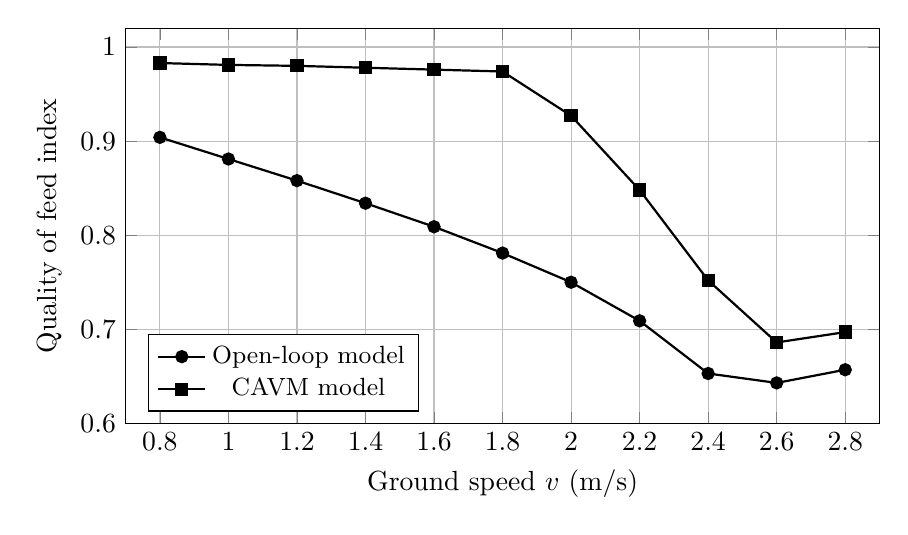
\begin{tikzpicture}
\begin{axis}[
  width=0.92\textwidth, height=6.6cm,
  xlabel={Ground speed \(v\) (m/s)},
  ylabel={Quality of feed index},
  xmin=0.7, xmax=2.9, ymin=0.6, ymax=1.02,
  grid=both, legend pos=south west, legend style={font=\small}
]
\addplot[thick, mark=*] coordinates {
(0.8,0.904) (1.0,0.881) (1.2,0.858) (1.4,0.834) (1.6,0.809)
(1.8,0.781) (2.0,0.750) (2.2,0.709) (2.4,0.653) (2.6,0.643) (2.8,0.657)
};
\addplot[thick, mark=square*] coordinates {
(0.8,0.983) (1.0,0.981) (1.2,0.980) (1.4,0.978) (1.6,0.976)
(1.8,0.974) (2.0,0.927) (2.2,0.848) (2.4,0.752) (2.6,0.686) (2.8,0.697)
};
\legend{Open-loop model, CAVM model}
\end{axis}
\end{tikzpicture}
\caption{Modelled quality-of-feed index against speed at zero acceleration, from Equations~\eqref{eq:openmiss} and \eqref{eq:closedmiss}. The closed-loop curve holds near \num{0.98} while repairs are timely and falls once Equation~\eqref{eq:cfrac} withdraws repair authority, then falls again through the timber resonance near \SI{2.4}{m/s}.}
\label{fig:qfi}
\end{figure}

Figure~\ref{fig:qfi} is a plot of the model, not of a trial. Two features are the ones the second technology will exploit. First, there is a wide plateau on which spending effort to go slightly faster buys almost no singulation loss and, as the energy model will show, almost no energy change, until the plateau ends. Second, the end is sharp. A planner that treats singulation as a linear penalty in speed will happily ride up to the cliff. A planner that treats \(\mathcal{V}_{\mathrm{meter}}\) as a hard set will stop at the plateau. Requirement~R3 chooses the hard set.

\subsection{Four rows, clocking and what the filter does not estimate}

The four row units are four copies of the same filter. They share the vehicle speed and the sample clock, and nothing else in the nominal design. Sharing the clock matters because a repair advance on row~1 and a repair advance on row~3 must not be queued on one processor so that the second repair misses its gate. The build therefore gives each row a detector thread with a reserved budget of \SI{22}{ms}, and it drops a frame rather than extending \(\tau_v\). A dropped frame lowers confidence, inflates the release-time process noise, and withholds repair for that hole. Withholding repair is the safe side of Borja's reversal.

Chassis coupling, neglected by Assumption~\ref{as:flex}, would appear as a common \(\delta\) component on all four rows when the whole machine pitches. The inertial sensors will see that common mode. A later revision can subtract the mean of the four \(\dot{\delta}\) estimates before the repair law runs. The present design does not. The estimation treats the omission as an unmodelled disturbance inside the process noise already scheduled by \(M(r)\), and it does not claim the four rows are independent in a statistical test. They are independent in the software architecture.

Seed identity across a double is not estimated. The filter counts a double. It does not decide which of the two seeds is the one that should have been released. For a single-species woody seed the distinction does not change the command. For a mixed-species restoration hopper it would, and that case is outside Assumption~\ref{as:seed}.

\subsection{A numerical pass through one empty cell}

The plate law is easier to audit on one hole than in the general notation. Take the design point \(v=\SI{1.4}{m/s}\), \(a=0\), \(x_{\mathrm{ref}}=\SI{0.20}{m}\) and \(N=24\). The hole period is
\begin{equation}
\label{eq:dtnum}
\Delta t = \frac{0.20}{1.4} = \SI{0.143}{s}.
\end{equation}
The feedforward plate speed is
\begin{equation}
\label{eq:omeganum}
\omega^{\star} = \frac{2\pi \cdot 1.4}{24 \cdot 0.20} = \SI{1.833}{rad/s},
\end{equation}
which is \num{17.5} revolutions per minute. One cell pitch is \(2\pi/24=\SI{0.262}{rad}\). The latency sum is \(\tau=\SI{0.057}{s}\), so
\begin{equation}
\label{eq:cnum}
1.35\tau + 0.030 = \SI{0.107}{s} < 0.143~\text{s},
\end{equation}
and Equation~\eqref{eq:cfrac} returns \(c=1\). A repair is allowed.

Suppose the detector, at a frame whose exposure began \SI{90}{ms} before the empty cell reaches the gate, returns an empty label with high confidence, and the flexure residual does not explain the absence. The remaining time before the gate, after inference, is about \(90-22=\SI{68}{ms}\). The stepper must gain one pitch in that window if the following cell is to arrive at the original gate time. The extra angular speed, held for those \SI{68}{ms}, is
\begin{equation}
\label{eq:domega}
\Delta\omega = \frac{0.262}{0.068} = \SI{3.85}{rad/s},
\end{equation}
about twice the feedforward. The actuator budget \(\tau_a=\SI{35}{ms}\) is the time to begin the move, not the time to finish a two-fold speed change if the following cell is still far away. In this numerical hole the following cell is one pitch behind, so the move is exactly the one-pitch advance of Equation~\eqref{eq:repair}, and \SI{68}{ms} is longer than \SI{35}{ms}. The repair fits. The same arithmetic at \(v=\SI{2.2}{m/s}\) gives \(\Delta t=\SI{0.091}{s}\) and \(c=0.55\), and the plate law withholds the advance. The empty cell becomes a miss that is logged and is not ``fixed'' by a late seed dropped into the next interval.

The flight that follows a successful release is independent of that logic and still has to be accounted for in the seed map. With \(H=\SI{0.42}{m}\) and negligible vertical release speed,
\begin{equation}
\label{eq:tfnum}
t_f = \sqrt{2\cdot 0.42/9.81} = \SI{0.293}{s}.
\end{equation}
At \SI{1.4}{m/s} the machine travels \(1.4\cdot 0.293=\SI{0.410}{m}\) during the flight. The tube and the furrow closer are built to cancel that mean transport, so the nominal landing sits on the target spacing. What they cannot cancel is a gate velocity that changes from seed to seed. An arm velocity \(\dot{\delta}=\SI{0.04}{m/s}\), which is a modest fraction of the resonant motion in Table~\ref{tab:speed}'s dynamic amplitude, shifts the landing by
\begin{equation}
\label{eq:jitternum}
\dot{\delta}\, t_f = 0.04\cdot 0.293 = \SI{11.7}{mm}.
\end{equation}
Relative to a \SI{200}{mm} spacing that jitter is a coefficient of variation contribution of about \num{0.06} if it is the dominant random term, which is inside the single class of Equation~\eqref{eq:classes} and is exactly why \(\mathrm{CV}_s\) is reported separately from \(\qfi\). The filter's \(v_{\mathrm{ex}}\) state exists so that this \SI{11.7}{mm} is written into the seed map rather than absorbed into a story about the plate having been wrong.

Depth on the same hole uses the static and dynamic pieces separately, as Proposition~\ref{prop:split} requires. The \SI{80}{N} mean soil force on \(k=\SI{8200}{N/m}\) is a \SI{9.8}{mm} offset. The integral term in Equation~\eqref{eq:depth} is what removes it; the open-loop column of the later tables leaves a \SI{4}{mm} remnant of that offset as the bias inside Equation~\eqref{eq:deptherr}. The roughness amplitude at this speed is \(d_{\mathrm{mm}}(1.4)=\SI{5.31}{mm}\). The servo rejection factor at a disturbance frequency \(1.4/0.45=\SI{3.11}{Hz}\), just under the \SI{3.2}{Hz} knee, is
\begin{equation}
\label{eq:etaz}
\eta_z = 0.30 + 0.08\cdot(1.4/2) = 0.356,
\end{equation}
so the rejected dynamic part is \(5.31\cdot 0.356=\SI{1.89}{mm}\). Combined with the \SI{1}{mm} residual bias,
\begin{equation}
\label{eq:sznum}
\sigma_{z,\mathrm{cl}} = \sqrt{1.89^2 + 1^2} = \SI{2.14}{mm},
\end{equation}
which is the closed-loop entry at \SI{1.4}{m/s} in the speed table of Chapter~\ref{ch:estimate}. The point of writing it here is that the table is not a separate experiment. It is Equation~\eqref{eq:sznum} evaluated on a grid.

\subsection{One unscented step on a reduced flexure state}

The five-dimensional filter is the one that runs. A two-dimensional reduction is the one a reader can check by hand, and it uses the same weights. Keep only \(\delta\) and \(\dot{\delta}\), with a predicted mean \(\hat{\delta}=\SI{2}{mm}\), \(\hat{\dot{\delta}}=\SI{0.01}{m/s}\), and a diagonal covariance \(P=\diag(10^{-6},\, 4\cdot 10^{-4})\) in metres and metres per second. Then \(n_x=2\), \(\lambda_{\mathrm{ukf}}=\alpha_{\mathrm{ukf}}^2 n_x - n_x\) with \(\alpha_{\mathrm{ukf}}=10^{-2}\), so \(\lambda_{\mathrm{ukf}}\approx -1.9998\) and \(n_x+\lambda_{\mathrm{ukf}}\approx 2\cdot 10^{-4}\). The sigma-point spread is small, which is what a small \(\alpha_{\mathrm{ukf}}\) is for: the points stay near the mean and the approximation remains local \cite{julier1997}. Over a \SI{10}{ms} step with \(F_{\mathrm{act}}\) cancelling the mean of \(F_{\mathrm{soil}}\) and with the linear stiffness, each point moves by
\begin{equation}
\label{eq:euler}
\begin{aligned}
\delta^{+} &= \delta + h_f \dot{\delta},\\
\dot{\delta}^{+} &= \dot{\delta} + h_f m_{\mathrm{eq}}^{-1}\bigl(F_{\mathrm{soil}}-c_d\dot{\delta}-k\delta\bigr).
\end{aligned}
\end{equation}
With \(h_f=\SI{0.01}{s}\) the mean displacement advances by \(10^{-4}\)~m, a tenth of a millimetre, and the mean velocity is pulled back toward zero by the stiffness term \(k\hat{\delta}/m_{\mathrm{eq}} = 8200\cdot 0.002/6.8 \approx \SI{2.41}{m/s^2}\), times \(h_f\), a change of about \(\SI{0.024}{m/s}\) before damping. Damping \(c_d\dot{\delta}/m_{\mathrm{eq}}\) at the predicted velocity is only about \(\SI{0.056}{m/s^2}\), so on this particular step stiffness dominates damping. The numerical content of the step is ordinary. What the unscented construction adds, and what an extended filter would approximate with one Jacobian, is that a sigma point sitting \SI{1}{mm} higher sees a different stiffness force and the predicted covariance of velocity grows in the direction the stiffness pushes. Process noise is then added on the diagonal, inflated by the magnification schedule when \(M(r)\) is large, and the ultrasonic update pulls \(\delta\) toward Equation~\eqref{eq:range}. The implementation note that matters for the build is the period: this step is cheap beside the detector, and it is the reason the filter runs at \SI{100}{Hz} while the camera runs at \SI{30}{Hz}. Between frames the release-time coordinate simply counts down, as Equation~\eqref{eq:trel} says, and the flexure coordinates keep integrating force.

\subsection{Vacuum margin and the cases the plate law refuses}

If the plate is pneumatic, Equation~\eqref{eq:vacuum} is evaluated at the edge of \(\mathcal{V}_{\mathrm{meter}}\) rather than at the working speed, so that a brief excursion inside the feasible set does not drop seeds the nominal vacuum cannot hold. Take a design seed of mass \(m_s=\SI{18}{mg}=\SI{1.8e-5}{kg}\) and an orifice area \(A_o=\SI{4}{mm^2}=\SI{4e-6}{m^2}\). The ratio \(m_s/A_o=\SI{4.5}{kg/m^2}\). At plate radius \(r_p=\SI{0.12}{m}\) and \(\omega^{\star}=\SI{1.833}{rad/s}\), the centripetal acceleration is \(r_p\omega^2\approx\SI{0.40}{m/s^2}\), small beside gravity. The vibration term is not small beside gravity once magnification grows. An arm acceleration of order \((2\pi f)^2\) times a few millimetres, at \(f=\SI{3}{Hz}\) and amplitude \SI{5}{mm}, is
\begin{equation}
\label{eq:avib}
a_{\mathrm{vib}} \approx (2\pi\cdot 3)^2 \cdot 0.005 \approx \SI{1.8}{m/s^2},
\end{equation}
about \(0.18\,g\). The holding pressure at the plateau edge is then of order
\begin{equation}
\label{eq:dpnum}
\Delta p \ge 4.5 \cdot (9.81 + 0.40 + 1.8) \approx \SI{54}{Pa}
\end{equation}
before orifice efficiency, seal leakage and the extra factor a real vacuum model puts on seed shape \cite{karayel2004}. Fifty pascals is a small gauge pressure. The practical content of the calculation is the opposite of its magnitude. Because the required pressure is small, operators turn the blower up until doubles appear, which is the ridge Singh, Singh and Saraswat mapped for cotton \cite{singh2005}. The vision loop's double term exists because the pressure that guarantees a pickup of the lightest seed in the lot also picks up a second seed when two small seeds cover one orifice. The nominal \(\Delta p\) is set with the \(a_{\mathrm{vib}}\) margin included, and the slow outer trim is allowed to lower it only when the logged double rate exceeds the logged miss rate for ten metres. It is not allowed to chase a single double with a pressure step inside one hole period. A wooden hopper's plenum, if a plenum is fitted at all, does not settle that fast.

The plate law also refuses three situations that look, from a distance, like opportunities to be clever. It refuses a repair when the hopper-level sensor on that row is low, because advancing the plate cannot fill a cell from an empty sector and the advance would only desynchronise the schedule. It refuses a repair when the realised delay, measured from exposure stamp to stepper issue, has exceeded the budget for three consecutive holes, because the \(c\) computed from the specification would otherwise keep authorising repairs the hardware is no longer fast enough to perform. It refuses to increase vacuum and plate speed in the same hole. Each of those actions can reduce misses and each of them can manufacture doubles. Stacking them on one observation is how a correct detector produces the sign change Borja measured \cite{borja2021}. One action per hole, and no action when \(c\) is low, is the rule the numerical hole above was written to illustrate.

\section{Singulation-constrained terrain model-predictive coverage}
\label{sec:tech2}

\subsection{Decisions the coverage technology is allowed to make}

Singulation-constrained terrain model-predictive coverage makes two decisions. Before work, or whenever the machine stops long enough to replan, it chooses a heading \(\beta\) relative to the uphill direction and a steady working speed \(v_{\mathrm{work}}\in\mathcal{V}_{\mathrm{meter}}\). During work it tracks the resulting swaths and is allowed to vary speed inside the horizon, including a reduction below \(v_{\mathrm{work}}\) when a headland acceleration would otherwise push \(c(v,a)\) down or when a local grade would push the flexure. It is not allowed to exceed the upper end of \(\mathcal{V}_{\mathrm{meter}}\), and it is not allowed to retune the miss model. The miss model is Equations~\eqref{eq:openmiss}--\eqref{eq:deptherr}, evaluated with the closed-loop branch because the meter on the machine is the meter of Section~\ref{sec:tech1}.

The technology is split into an outer coverage program and an inner quadratic-program tracker, following the time-scale split already argued for the joint problem. The outer program is allowed seconds. The inner program is required to finish inside the \SI{100}{ms} of Requirement~R7.

\subsection{Work model on a grade}

The mechanical work in Definition~\ref{def:p2} counts only the non-conservative part. A vehicle that drives up a slope and later drives down it returns the gravitational potential. What it does not return is the work against rolling resistance, the work dissipated in slip, and the aerodynamic drag, which at these speeds is small but is kept so that the model does not claim drag is zero. With vehicle mass \(M\), rolling coefficient \(C_{rr}\), a slip coefficient \(C_s\), drivetrain efficiency \(\eta_d\), air density \(\rho\), and drag area \(C_dA\),
\begin{equation}
\label{eq:fpm}
\begin{aligned}
\Gamma(\beta) &= 1 + \gamma\cos^2\beta,\\
F(v,\beta) &= C_{rr} Mg\cos\alpha + C_s Mg\sin^2\alpha\;\Gamma(\beta) + \tfrac12\rho\, C_dA\, v^2,\\
P(v,\beta) &= F(v,\beta)\, v / \eta_d .
\end{aligned}
\end{equation}
The heading \(\beta=0\) points uphill and \(\beta=\ang{90}\) lies on the contour. The factor \(\Gamma\) is larger when the vehicle points up the slope, because that is when the tangential weight, and therefore the slip loss, is organised against the motion rather than across it. The coefficients used in the estimation are \(M=\SI{460}{kg}\), \(C_{rr}=0.085\), \(C_s=2.0\), \(\gamma=1.15\), \(\eta_d=0.70\), \(\rho=\SI{1.15}{kg/m^3}\) and \(C_dA=\SI{0.85}{m^2}\). They are chosen so that a change of heading on an \num{8}\% grade changes work by several percent, which is the same order as the \numrange{9.5}{15.6}\% direction effect reported on the fields of Vahdanjoo, Gislum and S{\o}rensen, without copying a percentage from those fields onto this rectangle \cite{vahdanjoo2023}. A softer tyre or a wetter soil would raise \(C_{rr}\) and \(C_s\) together. The estimation does not sweep that change; it records the coefficients so that a later bench test of rolling resistance can replace them without touching the optimiser.

Headland distance is not free. A turn of radius \(R_{\mathrm{turn}}=\SI{4.2}{m}\) at the end of each swath contributes length \(\pi R_{\mathrm{turn}}\) and is driven at \SI{0.8}{m/s}, with an extra \num{8}\% on the force to represent the side-slip of the turn. If a heading produces \(n\) swaths of length \(L_{\mathrm{row}}\),
\begin{equation}
\label{eq:work}
W_{\mathrm{mech}} = \frac{F(v_{\mathrm{work}},\beta)}{\eta_d}\, n L_{\mathrm{row}} + 1.08\,\frac{F(0.8,\beta)}{\eta_d}\, n\pi R_{\mathrm{turn}}.
\end{equation}
Time is \(T = n L_{\mathrm{row}}/v_{\mathrm{work}} + n\pi R_{\mathrm{turn}}/0.8\). The number of swaths is \(n=\lceil S_{\perp}/w\rceil\) with swath width \(w=\SI{2.4}{m}\) and \(S_{\perp}\) the field width measured across the heading. On the estimation field the uphill heading has long rows and \(n=34\) turns, while the contour heading has short rows and \(n=75\) turns. Equation~\eqref{eq:work} therefore punishes the contour with turn work and turn time, and punishes the uphill heading with \(\Gamma(0)=1+\gamma\). That is the trade the outer program exists to settle. A planner that minimises only \(W_{\mathrm{mech}}\) will lean toward the contour. A planner that also counts failed seeds during the accelerations at each of \(75\) turns will lean back.

\begin{figure}[ht]
\centering
\begin{tikzpicture}[scale=0.95, font=\small, >=Stealth]
  \draw[thick] (0,0) rectangle (3.2,7.2);
  \node[rotate=90] at (-0.45,3.6) {uphill, long rows};
  \foreach \x in {0.3,0.7,...,2.9} {
    \draw[blue!70!black] (\x,0.25) -- (\x,6.95);
  }
  \draw[->] (3.5,0.3) -- (3.5,1.5) node[midway, right] {grade};
  \begin{scope}[xshift=6.4cm]
    \draw[thick] (0,0) rectangle (7.2,3.2);
    \node at (3.6,-0.45) {contour, short rows, many turns};
    \foreach \y in {0.28,0.68,...,2.9} {
      \draw[orange!80!black] (0.25,\y) -- (6.95,\y);
    }
    \draw[->] (7.5,0.2) -- (7.5,1.2) node[midway, right] {grade};
  \end{scope}
\end{tikzpicture}
\caption{The same rectangle covered along the slope and along the contour. Long uphill rows pay a sustained slip loss. Short contour rows pay a turn, and an acceleration, at every swath.}
\label{fig:field}
\end{figure}

The distance spent accelerating at each end of a swath is estimated as \(v_{\mathrm{work}}^2/(2a_{\mathrm{turn}})\) on entry and the same on exit. With \(a_{\mathrm{turn}}=\SI{0.7}{m/s^2}\), the fraction of row length spent at elevated acceleration is
\begin{equation}
\label{eq:frac}
\phi_{\mathrm{acc}} = \min\Bigl(1,\; \frac{n\, v_{\mathrm{work}}^2 / a_{\mathrm{turn}}}{n L_{\mathrm{row}}}\Bigr)
= \min\Bigl(1,\; \frac{v_{\mathrm{work}}^2}{a_{\mathrm{turn}} L_{\mathrm{row}}}\Bigr).
\end{equation}
Short rows make \(\phi_{\mathrm{acc}}\) large. The indices that enter the cost are the mixture
\begin{equation}
\label{eq:mix}
\mis = (1-\phi_{\mathrm{acc}})\,\mis_{\mathrm{cl}}(v,0) + \phi_{\mathrm{acc}}\,\mis_{\mathrm{cl}}(v,a_{\mathrm{turn}}),
\end{equation}
and likewise for multiples and for the depth error, with an extra \SI{0.6}{mm} on the depth error during the accelerated fraction to represent pitch into the headland. Equation~\eqref{eq:fail} then supplies \(\rho_{\mathrm{fail}}\). The seed count is \(N_{\mathrm{seed}} = 4\, n L_{\mathrm{row}} / x_{\mathrm{ref}}\), four rows along the same swath length.

\subsection{Outer program}

The outer program searches a finite set. Headings are taken at five-degree steps from \ang{0} to \ang{90}, using the symmetry of a rectangular field with a single slope direction. Speeds are taken at \SI{0.1}{m/s} steps inside \(\mathcal{V}_{\mathrm{meter}}\), with the resonant interval \([\SI{2.15}{m/s},\SI{2.55}{m/s}]\) removed even if a future change of \(x_{\mathrm{ref}}\) were to widen the latency set. For each candidate the cost of Definition~\ref{def:p2} is evaluated in closed form from Equations~\eqref{eq:work}--\eqref{eq:mix}. Infeasible candidates, those with modelled \(\qfi<0.955\) or \(\sigma_z>\SI{4}{mm}\), are discarded before the cost is compared. This is a lexicographic filter in front of a scalar cost, and it implements Requirements~R1 and~R2 as constraints rather than as terms that a weight could bargain away.

The weights used for the scalar comparison are \(w_T=\SI{0.55}{MJ/h}\) and \(w_s\) such that the failure term enters as \(4.0\,\rho_{\mathrm{fail}}\) in megajoule units on this field. The weights are planning preferences. They say that an hour of machine time is worth a fraction of a megajoule of the work budget, and that a failed placement is expensive relative to the energy differences, which are themselves only a few tenths of a megajoule. A user who prices contractor time higher can raise \(w_T\). The constraint filter does not move when the weights move. That separation is intentional. It keeps a cheap hour from buying a resonant speed.

For a non-rectangular field the same cost is evaluated along a coverage produced by the trapezoidal decomposition of Oksanen and Visala, or by the three-dimensional decomposition of Jin and Tang when the elevation model is not a single plane \cite{oksanen2009,jin2011}. The rectangle in the estimation is a plane of constant \(\alpha\), so the decomposition adds no region boundary and the heading search is the whole outer program. The algorithm is written for the general case so that a polygonal field does not require a different controller, only a different enumeration of swaths.

\begin{algorithm}[ht]
\caption{Heading and working-speed selection}
\label{alg:outer}
\begin{algorithmic}[1]
\Require polygon, elevation model, \(\mathcal{V}_{\mathrm{meter}}\), weights, index limits
\State build a swath set for each heading \(\beta\) in the candidate grid
\For{each \((\beta, v)\) with \(v\in\mathcal{V}_{\mathrm{meter}}\) outside the resonant interval}
  \State compute \(W_{\mathrm{mech}}\), \(T\), \(\phi_{\mathrm{acc}}\), \(\mis\), \(\mul\), \(\sigma_z\), \(\rho_{\mathrm{fail}}\)
  \If{\(\qfi \ge 0.955\) and \(\sigma_z \le \SI{4}{mm}\)}
    \State \(J \gets W_{\mathrm{mech}} + w_T T + w_s N_{\mathrm{seed}}\rho_{\mathrm{fail}}\)
    \State keep \((\beta,v)\) if \(J\) improves the incumbent
  \EndIf
\EndFor
\State \Return incumbent heading, speed, and the smoothed swath references
\end{algorithmic}
\end{algorithm}

Smoothing of the swath-to-swath join follows Graf Plessen and Bemporad: straight swaths are joined by a curvature-continuous turn whose curvature stays inside \(1/R_{\mathrm{turn}}\) and whose curvature rate stays inside the steering-rate limit \cite{plessen2017}. The speed profile along the join is then reduced, if needed, until \(c(v,a)\ge 0.85\) at every sample of the join. If no speed profile inside \(\mathcal{V}_{\mathrm{meter}}\) meets that test, the outer program lengthens the headland rather than violating the test. Lengthening the headland costs unplanted area at the field edge, which is already the usual price of a turning region \cite{bochtis2008}. The unplanted area is added to the miss term of those edge seeds so that a planner cannot hide a singulation problem by calling it headland.

\subsection{Inner tracker}

The inner tracker follows the smoothed reference with a linear time-varying model-predictive controller. The state and input are
\begin{equation}
\label{eq:xu}
\mathbf{x}_v =
\begin{bmatrix} x & y & \theta & v \end{bmatrix}^{\mathsf{T}},\qquad
\mathbf{u} =
\begin{bmatrix} \delta & a \end{bmatrix}^{\mathsf{T}}.
\end{equation}
The continuous kinematics are Equation~\eqref{eq:bicycle} together with \(\dot{v}=a\). Along a reference \((\mathbf{x}_{v,d},\mathbf{u}_d)\) the discrete linearisation at period \(h=\SI{100}{ms}\) is
\begin{equation}
\label{eq:ltv}
\mathbf{x}_{k+1} - \mathbf{x}_{v,d,k+1} = A_k (\mathbf{x}_k-\mathbf{x}_{v,d,k}) + B_k (\mathbf{u}_k-\mathbf{u}_{d,k}),
\end{equation}
with \(A_k\) and \(B_k\) the standard Jacobian of the bicycle, evaluated on the reference, exactly as in the agricultural linear time-varying trackers \cite{plessen2017}. The horizon is \(N_h=15\) steps, hence \SI{1.5}{s}, which at \SI{1.4}{m/s} looks \SI{2.1}{m} ahead, a little more than one turn radius of preview if the reference curvature is already rising.

The stage cost is not a pure tracking cost. With \(\tilde{\mathbf{x}}=\mathbf{x}-\mathbf{x}_{v,d}\) and \(\tilde{\mathbf{u}}=\mathbf{u}-\mathbf{u}_d\),
\begin{equation}
\label{eq:stage}
\begin{aligned}
\ell_k &= \tilde{\mathbf{x}}_k^{\mathsf{T}} Q \tilde{\mathbf{x}}_k + \tilde{\mathbf{u}}_k^{\mathsf{T}} R \tilde{\mathbf{u}}_k + w_{\rho}\,\rho_{\mathrm{fail}}\bigl(v_k,a_k,\sigma_z(v_k)\bigr) \\
&\quad + w_{M}\,\psi_{\mathrm{res}}(v_k).
\end{aligned}
\end{equation}
The resonance penalty \(\psi_{\mathrm{res}}\) is zero outside \([\SI{2.15}{m/s},\SI{2.55}{m/s}]\) and rises as a quadratic bowl inside it, centred on the speed where \(r=1\). It is a soft version of a constraint the outer program already enforced, repeated in the inner loop so that a disturbance that pushes the speed up cannot cross the bowl without paying. The hard constraints are
\begin{equation}
\label{eq:hard}
\begin{aligned}
&v_k \in \mathcal{V}_{\mathrm{meter}},\qquad
|a_k| \le a_{\max},\qquad
|\delta_k| \le \delta_{\max},\qquad
|\delta_k-\delta_{k-1}| \le \dot{\delta}_{\max}\, h,\\
&c(v_k,a_k) \ge 0.85.
\end{aligned}
\end{equation}
The last of these is linear in \(1/v\) and in \(|a|\) inside each piece of Equation~\eqref{eq:cfrac}, and it is implemented by two linear inequalities on each piece, selecting the piece from the reference speed. The fail term \(\rho_{\mathrm{fail}}\) is convex and increasing in \(|a|\) and, inside the plateau of Figure~\ref{fig:qfi}, nearly flat in \(v\). On the plateau it is approximated by its value at \(v_{\mathrm{work}}\) plus a linear slope taken from the model, which preserves convexity of the quadratic program. Near the boundary of \(\mathcal{V}_{\mathrm{meter}}\) the hard constraint is doing the work and the linear slope is only a tie-break. The quadratic program is solved with qpOASES \cite{ferreau2014}. The linearisation and the constraint matrices are formed with CasADi in the estimation and would be formed by the same generated code on the machine \cite{andersson2019}.

Terminal ingredients follow Mayne, Rawlings, Rao and Scokaert in reduced form \cite{mayne2000}. The terminal cost is the infinite-horizon cost of the linear quadratic regulator computed on the straight-swath linearisation, and the terminal set is a sublevel set of that cost on which the hard constraints are inactive. On a straight swath this is the classical construction. On a turn the reference is already feasible by the smoothing step, and the terminal set is replaced by a terminal equality to the reference at step \(N_h\), which is conservative and cheap. Recursive feasibility is then the statement that a feasible solution shifted by one step, with the terminal law appended, remains feasible. It holds while the disturbance in \(v\), from slip on the grade, stays inside the margin between \(v_{\mathrm{work}}\) and the boundary of \(\mathcal{V}_{\mathrm{meter}}\). The outer program is required to leave that margin. At the design point \(v_{\mathrm{work}}=\SI{1.4}{m/s}\) and the latency boundary near \SI{1.87}{m/s}, the margin is about \SI{0.47}{m/s}, which is larger than the speed error a \num{8}\% grade produces under the rolling-resistance model. If a steeper patch consumes the margin, the inner law brakes. Braking is always feasible inside Equation~\eqref{eq:hard} because lower speed improves \(c(v,a)\) and moves away from the resonance.

\begin{proposition}
\label{prop:feas}
If the smoothed reference lies in the interior of Equation~\eqref{eq:hard} and the one-step slip disturbance is bounded by the speed margin, the shifted warm-start remains feasible and the vehicle speed never settles inside the resonant interval.
\end{proposition}

The proof is the standard shifted-sequence argument of \cite{mayne2000} applied to a constraint set that does not depend on the measured singulation. The resonant interval is excluded by construction of \(\mathcal{V}_{\mathrm{meter}}\) and by \(\psi_{\mathrm{res}}\), not by an on-line estimate of seed spacing. That choice is deliberate. An on-line estimate of spacing arrives one flight time late, about \SI{0.29}{s} after release, and is the wrong signal to use as a hard constraint that must be feasible at the current step. The on-line spacing estimate is logged for the seed map \cite{griepentrog2005,ehsani2004}. It is not placed inside Equation~\eqref{eq:hard}.

\begin{figure}[ht]
\centering
\begin{tikzpicture}[font=\small, >=Stealth]
  \draw[thick] (0,0) -- (10,0);
  \draw[blue!70!black, thick] plot[smooth] coordinates {(0,0.1) (2,0.15) (4,0.55) (6,1.05) (8,1.15) (10,1.2)};
  \draw[dashed] (0,0) -- (10,0.15);
  \foreach \x in {0,1.3,2.6,3.9,5.2} {
    \draw[orange!80!black, ->] (\x,0) -- (\x+1.15,0.22);
  }
  \node[below] at (5,-0.15) {samples of the \SI{1.5}{s} horizon};
  \node[above] at (7.2,1.25) {reference};
  \node[anchor=west] at (0.2,1.5) {predicted speed stays off the resonant bowl};
\end{tikzpicture}
\caption{Inner horizon. Tracking error is penalised, and so is any predicted speed that approaches the timber resonance or any predicted acceleration that would make a repair late.}
\label{fig:horizon}
\end{figure}

\subsection{What the inner cost will not do}

Xu, Lai, Guo and Lu showed that a tracker allowed to care about efficiency can beat a tracker that only cares about path error, by \num{8.56}\% in their simulation \cite{xu2022}. The same freedom can be misused. If \(w_{\rho}\) is set to zero, Equation~\eqref{eq:stage} becomes a conventional tracker plus a weak resonance bowl, and a high \(w_T\) in the outer program will push \(v_{\mathrm{work}}\) to the boundary of the constraint. The design therefore keeps the index limits in the outer filter even when the weights change, and it keeps \(c(v,a)\ge 0.85\) as a hard inner constraint even when \(w_{\rho}\) is small. Efficiency is allowed to choose among admissible speeds. It is not allowed to define admissibility.

The inner program also does not schedule plate speed. Plate speed remains Equation~\eqref{eq:plate}, driven by the speed the vehicle actually has, not by the speed the planner wanted a second ago. Using the realised \(v\) closes the interface in the safe direction. If slip on the grade drops the realised speed, the plate slows and the spacing is held. If the planner's \(v_{\mathrm{work}}\) were sent straight to the plate while the wheels were still slow, the meter would bunch seeds at the start of every swath. Mangus's acceleration result is the field version of that bunching \cite{mangus2017}. Realised speed as the feedforward input is how the first technology protects itself from a confident plan.

Variable rate along a swath, in the precision-agriculture sense of a prescription map, fits the same interface. A prescription \(x_{\mathrm{ref}}(s)\) changes Equation~\eqref{eq:rate} and changes \(\Delta t\), and therefore changes \(\mathcal{V}_{\mathrm{meter}}\) locally, because a shorter spacing at the same speed is a shorter hole period. The outer program, if a prescription is present, evaluates \(c\) with the local spacing and lowers \(v_{\mathrm{work}}\) on the dense parts of the map. The estimation field uses a constant spacing, so this branch is specified and not exercised. It is the reason \(x_{\mathrm{ref}}\) is an input of Definition~\ref{def:p1} rather than a constant buried in the plate law.

\subsection{How the two technologies avoid a circular design}

There is an apparent circle. The metering technology publishes \(\mathcal{V}_{\mathrm{meter}}\) using \(\tau_v\), \(\tau_a\), \(f_n\) and \(\lambda\). The coverage technology chooses \(v\) inside that set and then drives the flexure at that \(v\), which is what \(f_n\) and \(\lambda\) were worried about. The circle is broken by the order of computation. The flexure parameters and the latency are properties of the hardware and of the detector. They do not depend on the heading. Equation~\eqref{eq:vset} can be evaluated before any coverage search. The coverage search never writes back into \(k\), \(\zeta\), \(\tau_v\) or \(\tau_a\). The only write-back is the realised speed, which the plate law accepts as an exogenous input. A fixed point is not being solved. A constraint computed from hardware is being obeyed by a planner.

The write-back that does exist is diagnostic. After a pass, the logged release times and the logged \(\hat{\delta}\) can update the estimate of \(f_n\) and of \(\lambda\), if the roughness of that field is not the design wavelength. The updated parameters change \(\mathcal{V}_{\mathrm{meter}}\) for the next pass. They are not allowed to change it in the middle of a hole period. This is the same discipline as the dropped-frame rule: a late adaptation is a worse fault than a slightly conservative speed.

\subsection{Arithmetic of the work model at two headings}

The outer program is a search over a closed form, so the closed form should be visible on one heading before Chapter~\ref{ch:estimate} prints a table of many. Take \(v=\SI{1.5}{m/s}\), grade \num{8}\% so \(\alpha=\arctan 0.08\) and \(\sin\alpha=\num{0.0797}\), \(\sin^2\alpha=\num{0.00636}\), and \(Mg=460\cdot 9.81=\SI{4513}{N}\). Rolling resistance is
\begin{equation}
\label{eq:frr}
C_{rr} Mg\cos\alpha = 0.085\cdot 4513\cdot 0.9968 = \SI{382}{N}.
\end{equation}
The slip term at a heading uses \(\Gamma(\beta)=1+1.15\cos^2\beta\). Uphill, \(\beta=0\), \(\Gamma=2.15\), and
\begin{equation}
\label{eq:fslip}
C_s Mg\sin^2\alpha\;\Gamma = 2.0\cdot 4513\cdot 0.00636\cdot 2.15 = \SI{123}{N}.
\end{equation}
At the contour, \(\beta=\ang{90}\), \(\Gamma=1\) and the slip term falls to \SI{57}{N}. Aerodynamic drag at \SI{1.5}{m/s} with \(C_dA=\SI{0.85}{m^2}\) and \(\rho=\SI{1.15}{kg/m^3}\) is \(\tfrac12\rho C_dA v^2\approx\SI{1.1}{N}\), which is why work barely moves when speed moves inside the plateau. Dividing by drivetrain efficiency \(\eta_d=0.70\) gives a force-per-metre, in energy units, of about \SI{724}{J/m} uphill and about \SI{630}{J/m} on the contour. Those are the values the estimation uses. They are not a dynamometer record.

On the rectangle, an uphill heading runs rows of \SI{180}{m} and needs \(n=\lceil 80/2.4\rceil=34\) swaths. Planting distance is \(34\cdot 180=\SI{6120}{m}\). Turn distance is \(34\cdot\pi\cdot 4.2\approx\SI{448}{m}\). Equation~\eqref{eq:work} then charges planting at the uphill force and turns at the lower turn speed with the eight-percent turn factor. The resulting work is \SI{4.78}{MJ}, which is the uphill entry the estimation table will show at this speed. A heading \ang{55} from uphill shortens the grade factor, increases the number of swaths, and lands near \SI{4.42}{MJ}. The difference, about \SI{0.36}{MJ}, is the whole energy prize available on this field. It is smaller than the energy a reader might expect from the phrase ``terrain-aware'', and it is large enough, against a time weight of \SI{0.55}{MJ} per hour, that the optimiser will not ignore it. It is not large enough to justify leaving \(\mathcal{V}_{\mathrm{meter}}\). That comparison is the reason the index filter sits in front of the scalar cost rather than inside it.

The accelerated fraction on the long uphill rows at \SI{1.5}{m/s}, from Equation~\eqref{eq:frac} with \(a_{\mathrm{turn}}=\SI{0.7}{m/s^2}\), is
\begin{equation}
\label{eq:phi}
\phi_{\mathrm{acc}} = \frac{1.5^2}{0.7\cdot 180} = 0.018,
\end{equation}
under two percent of the row. On the short contour rows of \SI{80}{m} the same formula gives \(1.5^2/(0.7\cdot 80)=0.040\). Mixing the zero-acceleration and the turn-acceleration miss models with those weights, as Equation~\eqref{eq:mix} does, changes the closed-loop miss probability in the third digit at this speed. Heading is therefore not a singulation decision at \SI{1.5}{m/s}. It becomes one if someone proposes \(v=\SI{2.4}{m/s}\), where both the base miss model and the magnification are already bad on the straight, and the accelerated fraction makes them worse. The outer program never reaches that comparison as a cost trade, because the index filter has already discarded the candidate.

\subsection{Linearisation used by the inner tracker}

On a straight swath at \(v_d=\SI{1.4}{m/s}\), \(\theta_d=0\) and \(\delta_d=0\), the bicycle Jacobian with respect to \((x,y,\theta,v)\) and \((\delta, a)\), sampled at \(h=\SI{0.1}{s}\), is dominated by a simple structure. Position \(x\) integrates speed. Position \(y\) integrates \(v\theta\) for small heading error, so the discrete \(A\) carries a term \(h v_d\) from \(\theta\) into \(y\). Heading integrates \((v/\ell)\delta\) for small steering, so \(B\) carries \(h v_d/\ell\) from steering into heading, and from there, one step later, into lateral error. With a wheelbase \(\ell=\SI{1.6}{m}\),
\begin{equation}
\label{eq:jac}
\frac{\partial \dot{\theta}}{\partial \delta}\bigg|_{\delta=0} = \frac{v}{\ell} = \frac{1.4}{1.6} = \SI{0.875}{s^{-1}},
\end{equation}
and one tracker step of steering equal to \SI{0.05}{rad} changes heading by about \(0.875\cdot 0.05\cdot 0.1=\SI{0.0044}{rad}\), then changes lateral position on the following step by about \(1.4\cdot 0.0044\cdot 0.1\approx\SI{0.6}{mm}\). The tracker does not steer in one-step impulses of that size. The arithmetic shows why a \SI{1.5}{s} horizon is long enough to see a lateral error coming and short enough that the linearisation, recomputed each step on the reference, does not have to carry the vehicle around a full turn inside one linear model. The turn itself is in the reference, through the smoothing of Graf Plessen and Bemporad, and the linearisation is about that curved reference rather than about a straight line \cite{plessen2017}. Recomputing \(A_k\) and \(B_k\) every \SI{100}{ms} is the ``time-varying'' part of the linear time-varying controller. Freezing them for the whole headland would be a linear controller about the wrong point.

The quadratic weights used with this linearisation are diagonal,
\begin{equation}
\label{eq:QR}
\begin{aligned}
Q &= \diag(2,\, 8,\, 4,\, 1),\\
R &= \diag(0.4,\, 0.3),
\end{aligned}
\end{equation}
on states in metres, radians and metres per second, and on inputs in radians and metres per second squared. Lateral error is weighted more heavily than longitudinal error because a row that has drifted by ten centimetres plants the neighbouring row's strip, whereas a longitudinal lag of ten centimetres is removed by the plate law as soon as the realised speed is known. Speed error is weighted lightly inside \(Q\) because speed is already constrained by Equation~\eqref{eq:hard}, and a large speed weight would fight the resonance bowl and the repair constraint with an objective they have already settled. These weights are part of the specification of the inner tracker. They are not identified from a human driver.

A warm start for qpOASES is the previous solution with the first move discarded and the terminal linear-quadratic move appended \cite{ferreau2014,mayne2000}. On a straight swath the active set is usually empty: the inequalities are slack by the margin the outer program left, about \SI{0.47}{m/s} between \SI{1.4}{m/s} and the latency boundary near \SI{1.87}{m/s}. The solver then returns in a few factorisations. The \SI{40}{ms} budget in the build is set for the worse case, a headland in which the acceleration inequality and the repair inequality are both close to active. If a solve exceeds the budget, the tracker applies the second move of the previous feasible solution and marks the step as a hold. A hold is feasible by the shifted-sequence argument of Proposition~\ref{prop:feas}. An infeasible scramble for a new solution is not.

\subsection{A local spacing change, and why the speed set moves with it}

A prescription that asks for \(x_{\mathrm{ref}}=\SI{0.12}{m}\) on one patch of the field, and \SI{0.20}{m} elsewhere, changes the hole period at the same ground speed from \SI{0.143}{s} to \(0.12/1.4=\SI{0.086}{s}\). Against the repair threshold of \SI{0.107}{s} from Equation~\eqref{eq:cnum}, the tighter spacing is no longer inside the full-repair set at \SI{1.4}{m/s}. The speed that restores \(\Delta t\ge\SI{0.107}{s}\) is
\begin{equation}
\label{eq:vpresc}
v \le \frac{0.12}{0.107} = \SI{1.12}{m/s}.
\end{equation}
The outer program, on that patch, lowers the reference speed to \SI{1.1}{m/s} before the tracker runs. The plate law does not have to discover the violation by attempting repairs and then withdrawing them. This is the local form of Requirement~R10. One speed set, recomputed from the local spacing, is the only message the prescription is allowed to send into the tracker. A prescription that instead sent a plate speed directly would bypass the repair test and recreate, on the dense patch, the late-repair regime the whole design is built to avoid.

The same patch does not require a new heading. Heading was chosen for the field's grade and for the number of turns, neither of which the prescription changes. Replanning the heading because one patch wants a slower speed would rotate every other swath for a constraint that a speed change already satisfies. The inner tracker is allowed to deviate from \(v_{\mathrm{work}}\) inside the horizon. The outer heading stays put until the elevation model or the field boundary changes. That is a second time-scale split, inside the coverage technology, and it is why Algorithm~\ref{alg:outer} returns a single heading for the rectangle even though the tracker is free to slow down.

\subsection{What has been fixed for the estimation}

The estimation is allowed to evaluate, and is not allowed to revise, the following objects: the flexure parameters and the latency that define \(\mathcal{V}_{\mathrm{meter}}\); the miss and depth maps of Equations~\eqref{eq:openmiss}--\eqref{eq:deptherr}; the work coefficients inside Equation~\eqref{eq:fpm}; the weights \(w_T\) and the failure weight; the index thresholds \num{0.955} and \SI{4}{mm}; the resonant interval \([\SI{2.15}{m/s},\SI{2.55}{m/s}]\); and the tracker weights of Equation~\eqref{eq:QR}. Chapter~\ref{ch:estimate} may only choose which plans to place side by side and may only report the numbers those objects produce. The hardware chapter that precedes the tables exists so that a reader who doubts a latency or a sample period can see the task that is supposed to meet it, and can see which table entry moves if that task is slower than its budget.

\subsection{One headland, sample by sample}

The inner tracker is easiest to distrust in a turn, because that is where speed, acceleration and curvature change together and where Mangus and colleagues found the singulation errors organised themselves \cite{mangus2017}. Consider the exit from an uphill swath into a turn of radius \(R_{\mathrm{turn}}=\SI{4.2}{m}\) at the moment the reference begins to slow from \SI{1.4}{m/s} toward the turn speed \SI{0.8}{m/s}. The distance available for that slowing, if the reference is to arrive at the turn at \SI{0.8}{m/s} with \(a=-\SI{0.7}{m/s^2}\), is
\begin{equation}
\label{eq:brake}
\frac{v_1^2-v_2^2}{2|a|} = \frac{1.4^2-0.8^2}{1.4} = \SI{0.94}{m}.
\end{equation}
At a \SI{100}{ms} sample the vehicle covers about \SI{0.14}{m} at the start of the braking and about \SI{0.08}{m} at the end, so the manoeuvre occupies roughly eight to ten tracker steps, well inside the fifteen-step horizon. The horizon that begins a second and a half before the brake therefore already contains the whole speed change. The predicted accelerations are about \(-\SI{0.7}{m/s^2}\). Equation~\eqref{eq:cfrac} at \(v=\SI{1.4}{m/s}\) and \(|a|=\SI{0.7}{m/s^2}\) still returns \(c=1\), because the hole period is \SI{0.143}{s} and the acceleration surcharge \(0.012\cdot 0.7\approx\SI{0.008}{s}\) does not push the threshold above the hole period. The hard constraint is slack. The stage cost still penalises the acceleration through \(\rho_{\mathrm{fail}}\), but only by the mixture weight of a short distance, which is why \(\phi_{\mathrm{acc}}\) on the long rows stayed near two percent.

What the tracker must not do, and what a pure time-optimal tracker would do, is postpone the braking and then brake harder. A brake of \(\SI{1.2}{m/s^2}\) over a shorter distance would finish the swath earlier by a fraction of a second and would drop \(c\) toward the \num{0.71} computed earlier for that acceleration at a slightly higher speed. Equation~\eqref{eq:hard} forbids that brake even if the time weight would have liked it. The headland is therefore not an exception to the metering technology. It is the place the exception would have been, and the constraint is written there on purpose.

During the turn itself the plate may be inhibited by the boot-lift interlock if the headland is unplanted, which is the usual layout \cite{bochtis2008}. Inhibition is cleaner than asking the meter to singulate while the boot is out of the soil and the ultrasonic range is invalid. When the next swath begins, the integral of the depth loop is released from its freeze, the plate feedforward tracks the realised speed as the vehicle climbs back from \SI{0.8}{m/s} to \SI{1.4}{m/s}, and repairs are authorised only once \(c\) has returned. The first metre of the new swath is the other place a naive plan bunches seeds, by commanding the working plate speed before the wheels are at the working speed. Using realised \(v\) in Equation~\eqref{eq:plate} spreads that first metre at the correct spacing instead. The cost is a slightly later start of full-rate planting, already paid for in the headland length.

\subsection{Logging that makes the next pass stricter rather than braver}

Each release writes a row to the seed map: vehicle pose, filter release time, estimated exit velocity, detector label, repair flag, realised delay, and filtered depth. The row is an estimate, not a proof that a seed lies at the computed coordinate. Its first use is the one Griepentrog, N{\o}rremark, Nielsen and Blackmore described, a map a later operation can follow \cite{griepentrog2005}. Its second use is internal, and it is deliberately asymmetric. If the realised delay over a swath exceeds the budget, the next swath's \(\tau\) is raised and \(\mathcal{V}_{\mathrm{meter}}\) shrinks. If the delay is better than the budget, \(\tau\) is not lowered on the same day. A fast swath can be luck of the scheduler. A slow swath is evidence the inequality is tighter than the specification. The same asymmetry applies to \(f_n\). A resonance that appears in \(\hat{\delta}\) widens the forbidden interval for the next pass. A quiet swath does not delete the interval, because the roughness wavelength of one swath is not the wavelength of the field. Adaptation that only ever tightens the constraint cannot talk a machine into the regime Borja's loop entered when the processor fell behind \cite{borja2021}. Adaptation that updates in both directions can.

The log is also the object a later germination count has to be joined to, if the survival function \(S(\sigma_z)\) is ever replaced by a measured curve. Joining requires the landing coordinate from Equation~\eqref{eq:carry}, not only the vehicle coordinate at the moment the detector fired. Those two coordinates differ by the flight transport, about \SI{0.41}{m} at the design speed, which is two target spacings. A survival count joined to the wrong coordinate would teach the next version of the cost to fear the wrong places. The build therefore stores both stamps. None of this changes the quadratic program. It is the reason the release log is a row in the interface table and not an optional debug print.

\subsection{A calibration pass before the first planted swath}

The stiffness \(k\) is a specification of the timber link. The soil coefficient \(k_{\mathrm{soil}}\) in Equation~\eqref{eq:flinear} is not, because it belongs to the field. The build therefore begins a planting day with a calibration pass rather than with a planted swath. The pass is one swath length, plates disengaged, boot in the soil, depth screw held at three set-points around the \SI{18}{mm} target, for a few metres each. Boot force and ultrasonic depth are logged. The slope of force against depth is \(k_{\mathrm{soil}}\). A value of order a few newtons per millimetre is what the linearisation expects; the \SI{80}{N} static force at the target depth is the intercept \(F_0(z^{\star})\), and it is the number that produced the \SI{9.8}{mm} undeflected offset \(F_0/k\). If the calibration intercept is \SI{110}{N} rather than \SI{80}{N}, the undeflected offset is \(110/8200=\SI{13.4}{mm}\), still inside the screw travel, and the integral term is required to work harder. The filter does not need a new structure for that. It needs the new intercept written into \(F_{\mathrm{soil}}\) before the first repair is authorised.

The same pass estimates the roughness wavelength that the design took as \(\lambda=\SI{0.45}{m}\). The force residual after the linear depth term is removed is a time series along the swath. Its dominant spatial frequency, if one is visible, replaces \(\lambda\) in the magnification formula before \(\mathcal{V}_{\mathrm{meter}}\) is published. If the residual is broadband, the design wavelength is kept and the process noise on \(\delta\) stays on the magnification schedule already stated. Publishing \(\mathcal{V}_{\mathrm{meter}}\) after this pass, rather than from the workshop specification alone, is the one adaptation allowed before motion. It is still not an adaptation inside a hole period. The tracker does not move until the set has been published, which is the order of computation that broke the apparent circle between the two technologies.

A calibration that cannot be finished, because the ultrasonic return is invalid or the force signal is saturated, inhibits planting. The alternative is to run the design values and hope the field matches the specification. The interlock refuses that alternative. A wooden machine is light enough that an unexpected soil force moves the boot by millimetres, which is the whole reason the depth loop exists, and a depth loop without a force intercept is an integral winding up against an unknown load. The pass costs one swath of time, already small beside the \SI{1.4}{h} the estimation assigns to the field, and it is the price of keeping Equation~\eqref{eq:deptherr} attached to the soil under the machine rather than to the soil imagined in the problem set.

Table~\ref{tab:cal} is the decision the pass is allowed to make. The screw travel specified in the build has to cover the largest intercept in the table, \SI{24}{mm} of undeflected offset plus the \SI{18}{mm} target plus a lift clearance. An intercept of \SI{200}{N} is a stiffer or a deeper soil than the problem set assumed, and it is still a calibration result rather than a reason to abandon the flexure model. Only a saturated load cell, which cannot produce an intercept at all, inhibits the day. The resonant speed column shows the other output of the same pass. A shorter roughness wavelength moves the forbidden steady speed down, and the tracker inherits that number with the feasible set. No weight in the coverage cost is allowed to override the last column.

\begin{table}[ht]
\centering
\caption{Calibration outcomes the first pass may publish. Offsets use \(k=\SI{8200}{N/m}\). The resonant speed uses the measured wavelength in \(v \approx \lambda f_n\).}
\label{tab:cal}
\begin{tabular}{@{}rrll@{}}
\toprule
Intercept (N) & Offset (mm) & Measured \(\lambda\) (m) & Forbidden near (m/s) \\
\midrule
80 & 9.8 & 0.45 & 2.4 \\
110 & 13.4 & 0.45 & 2.4 \\
110 & 13.4 & 0.30 & 1.7 \\
200 & 24.4 & 0.60 & 3.3 \\
\bottomrule
\end{tabular}
\end{table}

The third row is the one that changes the plan rather than only the depth bias. A wavelength of \SI{0.30}{m} puts the resonance near \(0.30\cdot 5.53\approx\SI{1.66}{m/s}\), inside the plateau where the latency constraint would still have allowed \SI{1.4}{m/s} to \SI{1.8}{m/s}. The feasible set then has a hole where the magnification exceeds the bound used in Equation~\eqref{eq:vset}. The low side of that hole keeps the arm quiet and spends time. The high side is already where repair authority falls and where the \SI{3}{Hz} depth servo loses the roughness. On the estimation coefficients the index filter refuses the high side, and the machine plants more slowly than the \SI{1.4}{m/s} of Table~\ref{tab:plans} after a calibration that discovers short roughness. That is the correct refusal. A planner that kept \SI{1.4}{m/s} because the workshop wavelength had been \SI{0.45}{m} would be driving on the resonance the pass had just measured.

Chapter~\ref{ch:estimate} can now be a calculation rather than a narrative. The hardware that would host the calculation is specified first, so that the sample periods and the latency budget used above have a place to live. The calculation then evaluates Equations~\eqref{eq:openmiss}--\eqref{eq:work} on the field of the problem set, for the open-loop baselines and for the plan Algorithm~\ref{alg:outer} returns.
